\documentclass[fleqn]{jbook}
\usepackage{physpub}

\begin{document}
\begin{question}{専攻 問題4}{}
\begin{subquestions}
\SubQuestion
 図1はKelvinの電気秤であり、天秤LのおもりMの値を変化させることで、固定電極Aに加えた電圧を測定できる。



\begin{minipage}{.5\linewidth}
Bは接地された可動電極(極板面積$S$)、Gは接地されたガード電極(固定)でBの周囲を取り囲んでいる。A、Gの極板間隔を$d$、重力加速度を$g$、空気の誘電率は真空の誘電率$\varepsilon_{0}$と同じとして、以下の問いに答えよ。
\end{minipage}
\hspace*{.05\linewidth}
\begin{minipage}{.45\linewidth}
\begin{center}
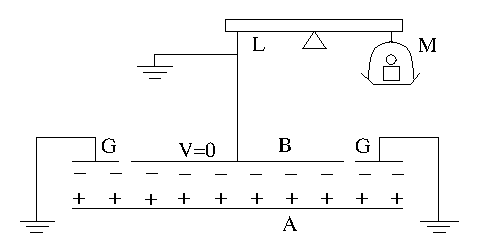
\includegraphics[clip,width=\linewidth]{1999phy4-1.eps}\\
図1
\end{center}
\end{minipage}

\begin{subsubquestions}
\SubSubQuestion
Aに加えた電圧$V$(Bに対する電位)を測定する手順を、実際に測定することを想定してなるべく詳しく記述し、$V$を求める式を導け。(ちなみに、Kelvinは実際にはAに既知の電位を与え誘電率$\varepsilon_{0}$を測定するためにこの秤を用いた。)
\SubSubQuestion
ガード電極Gを配置する意味を答えよ。

\end{subsubquestions}

\SubQuestion
受動回路素子(抵抗R、コンデンサーC、コイルL)のインピーダンスを正確に測定する方法にブリッジ法がある。この方法は、未知のインピーダンス$Z_{x}$と既知の(可変)インピーダンス$Z_{i}(i=1\sim 3)$を使い、ブリッジをバランスすることで$Z_{x}$を精密に測定する方法である。測定には必要に応じて周波数可変な信号源を用いることが出来るものとして、以下に答えよ。

\begin{subsubquestions}
\SubSubQuestion
理想的なコイル$\mathrm{L}_{x}$の未知のインダクタンス$L_{x}$を、既知の純抵抗$R_{1},R_{2},R_{3}$を用いてブリッジ法で測定するための回路図を示し、$L_{x}$を求める方法を解説せよ。
\SubSubQuestion
現実的には理想的な受動素子は存在せず、寄生成分と呼ばれる避けられないインピーダンス成分が存在する。
\begin{minipage}{.5\linewidth}
たとえばコイルのインダクタンス$\mathrm{L}_{i}$には、直列に巻線抵抗R${}_{i}$、並列に巻線間分布容量C${}_{i}$が存在する(図2)。(i)で考えた回路で用いたL${}_{x}$に寄生成分がある場合、寄生成分の値を推定する方法を簡潔に論じよ。
\end{minipage}
\hspace*{.05\linewidth}
\begin{minipage}{.45\linewidth}
\begin{center}
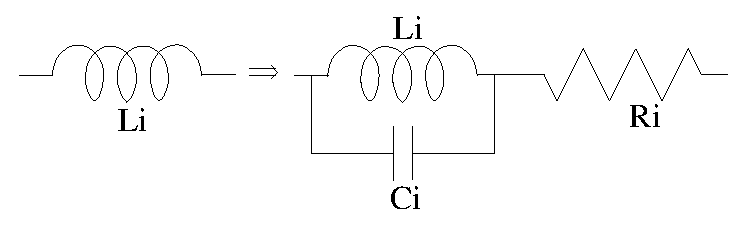
\includegraphics[clip,width=\linewidth]{1999phy4-2.eps}\\
図2
\end{center}
\end{minipage}
\end{subsubquestions}

\SubQuestion
太陽電池では、シリコンのpn接合部分にバンドギャップ(約0.6eV)よりも大きなエネルギーをもつ1個の光子が当たったときに電子−正孔が生じ、それらが界面電場により互いに逆方向にドリフトすることで、2つの電極間に光起電力が発生する。必要ならば、光速度$c=3.0\times 10^{8}$~[m/s]、素電荷$e=1.6\times 10^{-19}$~[C]、Planck定数$h=6.6\times 10^{-34}$~[J$\cdot$s]、Boltzman定数$k=1.4\times 10^{-23}$~[J/K]を用い、以下の問いに答えよ。

\begin{subsubquestions}
\SubSubQuestion
太陽電池に光を照射した際プラス極になるのは、p型、n型のどちらに接続した電極か。理由を付けて答えよ。

\SubSubQuestion
温度$T$~[K]の光源(黒体)の単位面積から単位時間に放出される電磁場の全輻射エネルギー$I$~[W/m${}^{2}$]は、$I=\sigma T^{4}$で与えられる。ここで$\sigma =5.7\times 10^{-8}$~[W/m${}^{2}$/K${}^{4}$]はシュテファンボルツマン定数である。今、太陽を温度$5.8\times 10^{3}$~[K]の黒体とした時、単位時間に太陽から放出される総輻射量$P_{0}$~[W]および地球軌道上(地球の大気圏外)における単位面積あたりの太陽輻射量$I_{0}$~[W/m${}^{2}$]を概算せよ。なお、太陽の半径は$7.0\times 10^{8}$~[m]、太陽までの距離は$1.5\times 10^{11}$~[m]である。

\SubSubQuestion
図3、4は、地球軌道上(地球の大気圏外)における単位面積あたりの太陽輻射光子数と標準的な太陽電池の量子効率を表している。このことから、5 cm $\times$ 5 cmの太陽電池を地球軌道上(地球の大気圏外)で太陽に正対して置き、両極を短絡したときに流れる電流量を見積もれ。

\SubSubQuestion
よく晴れた日に(iii)の太陽電池を地表に置き太陽に正対させて測定したところ、(iii)で見積もった結果の約65\%しか電流が流れなかった。この食い違いの原因を説明せよ。\\

\begin{minipage}{.5\linewidth}
\begin{center}
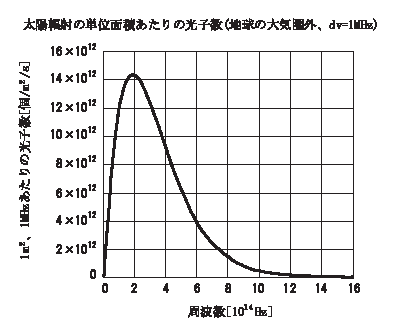
\includegraphics[clip]{1999phy4-3.eps}\\
図3
\end{center}
\end{minipage}
\begin{minipage}{.5\linewidth}
\begin{center}
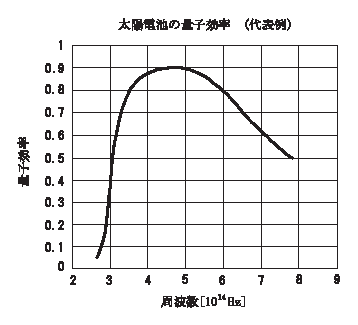
\includegraphics[clip]{1999phy4-4.eps}\\
図4
\end{center}
\end{minipage}
\end{subsubquestions}

\end{subquestions}
\end{question}
\begin{answer}{専攻 問題4}{}
\begin{subanswers}
\SubAnswer
\begin{subsubanswers}
\SubSubAnswer
まずAを接地し、その時点でAB間の距離が$d$であることを確かめる。次にBをAに接触しないように支えておきながら極板Aに電圧$V$を加える。BはAに引っ張られるので、おもりMを加減してAB間の距離が$d$になるように調節する。

電極Bの電荷を$Q_B$、電極Gの電荷を$Q_G$、面積を$S_G$、A,Bの極板間隔を$x$とすると
\begin{eqnarray}
 \frac{Q_B}{S} &=& \frac{\varepsilon_0 V}{x} \eqname{A4-1-1}\\
 \frac{Q_G}{S_G} &=& \frac{\varepsilon_0 V}{d} \eqname{A4-1-2}
\end{eqnarray}
である。
$x=d$であるから電極Bにかかるクーロン力は
\[
\frac{1}{2} Q_B E_{AB} = \frac{1}{2} \varepsilon_0 \frac{S}{d} V \frac{V}{d} = \frac{1}{2} \frac{\varepsilon_0 S V^2}{d^2}
\]
これと$Mg$が等しくなるように$M$を選べばよくて、
\[
\frac{1}{2}\frac{\varepsilon_0 SV^2}{d^2} = Mg
\]
\[
\therefore V=\sqrt{\frac{2Mg}{\varepsilon_0 S}}d
\]

\SubSubAnswer
Bの周辺において生じる静電界の不均一をなくす。また、AB間の距離を$d$にする目安になる。
\end{subsubanswers}

\SubAnswer
\begin{subsubanswers}
\SubSubAnswer
通常のブリッジ法は検流計に電流が流れなくなる様に可変抵抗でバランスを取るのであるが、ここではコイル1つ抵抗3つを使うという設定と思われるので、これらの素子をブリッジ法の各辺に配置しても平衡は成り立たない。そこで検流計に流れる電流を信号源の周波数を変えて測定する事により、インダクタンスを測定する(図5)。

\begin{minipage}{.5\linewidth}
\begin{align}
& Z_1 I_1 = Z_2 I_2 \eqname{A4-2-1}\\
& Z_4 (I_1 - I_3) = Z_3 (I_2 + I_3) \eqname{A4-2-2} \\
& Z_2 I_2 + Z_3(I_2 + I_3) = V_0 e^{i \omega t} \eqname{A4-2-3}
\end{align}
\\
$Z_4$にはコイルを配置する。すなわち、
\begin{eqnarray*}
&&Z_1 = R_1 \qquad Z_2 = R_2 \\
&&Z_3 = R_3 \qquad Z_4 = i \omega L_x
\end{eqnarray*}
\end{minipage}
\hspace{.2\linewidth}
\begin{minipage}{.3\linewidth}
\begin{center}
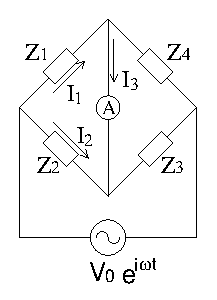
\includegraphics[clip,height=5cm]{1999phy4-5.eps}\\
図5
\end{center}
\end{minipage}
\eqhref{A4-2-1},\eqhref{A4-2-2}より
\begin{equation}
 I_2 = \frac{Z_1 (Z_3 + Z_4)}{Z_2 Z_4 - Z_1 Z_3} I_3 \eqname{A4-2-4}
\end{equation}

\eqhref{A4-2-3},\eqhref{A4-2-4}より
\begin{eqnarray*}
 I_3 &=& \frac{Z_2 Z_4 - Z_1 Z_3}{Z_1 Z_2 Z_3 +Z_2 Z_3 Z_4 +Z_3 Z_4 Z_1 +Z_4 Z_1 Z_2} V_0 e^{i \omega t} \\
 &\equiv& \frac{i \omega L_x R_2 - R_1 R_3}{R + i \omega L_x r} V_0 e^{i \omega t}
\end{eqnarray*}
(但し、$R \equiv R_1 R_2 R_3,\quad r \equiv R_1 R_2 + R_2 R_3 + R_3 R_1$)
\begin{eqnarray*}
 \therefore |I_3|^2 &=& \frac{{R_1}^2 {R_3}^2 + {R_2}^2 \omega ^2 {L_x}^2}{R^2 + \omega ^2 {L_x}^2 r^2} {V_0}^2 \\
 &=& \frac{{R_2}^2 + \frac{{R_1}^2 {R_3}^2}{\omega ^2 {L_x}^2}}{r^2 + \frac{R^2}{\omega ^2 {L_x}^2}} {V_0}^2 \quad \rightarrow \quad\frac{{R_2}^2}{r^2} {V_0}^2 \qquad (\omega \rightarrow \infty)
\end{eqnarray*}

$I_3$を、周波数$\omega$を変えながら測定しプロットする。その形を理論値と比較してフィッティングを行えば$L_x$を求めることができる($V_0$の値は$\omega \rightarrow \infty$ とすれば求めることができる)。

\SubSubAnswer
まず、巻線抵抗$R_i$を求める。\\
図5において直流電源をつなげば、検流計に電流が流れなくなった時、ブリッジ法の平衡の式より$R_i = \frac{R_1 R_3}{R_2}$となる。

\begin{minipage}{.5\linewidth}
次に図6のようにコイルと交流電源をつなぐ。現実のコイルのインピーダンスは
\begin{eqnarray*}
 Z &=& R_i + \frac{1}{\frac{1}{i \omega L_i} + i \omega C_i} \\
   &=& R_i + i \frac{\omega L_i}{1 - {\omega}^2 L_i C_i}
\end{eqnarray*}

${\omega}^2 = \frac{1}{L_iC_i}$で電流が最小になる。これによって$L_iC_i$の値がわかる。また、
\[
|Z| = \sqrt{{R_i}^2 +\left(\frac{\omega L_i}{1-{\omega}^2 L_i C_i}\right)^2 }
\]
だから、適当な$\omega$でインピーダンスを求めれば$R_i$, $L_i C_i$は分かっているので$L_i$が求まる。すると$C_i$もわかる。
\end{minipage}
\hspace{.1\linewidth}
\begin{minipage}{.2\linewidth}
\begin{center}
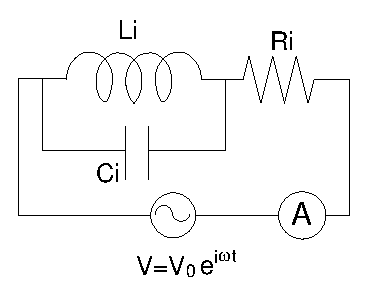
\includegraphics[clip,width=4cm]{1999phy4-6.eps}\\
図6
\end{center}
\end{minipage}

\end{subsubanswers}

\SubAnswer
\begin{subsubanswers}
\SubSubAnswer
答え:p型\\
\begin{minipage}{.5\linewidth}
理由:接合部付近は正孔と電子が吸収しあって、キャリアが存在しない層(空乏層:depletion layer)ができる(図7)。空乏層のp型部分ではアクセプタの電荷、つまり負電荷があらわれる。n型部分ではドナーの電荷、正電荷があらわれる。電荷分布は図8のようになるから、接合部付近ではn型$\rightarrow$p型の向きに電場が生じる。このため、光子が当たった時に生じる電子はn型方向に、正孔はp型方向に加速される。したがってp型がプラス極になる。
\end{minipage}
\hspace{.1\linewidth}
\begin{minipage}{.4\linewidth}
\begin{center}
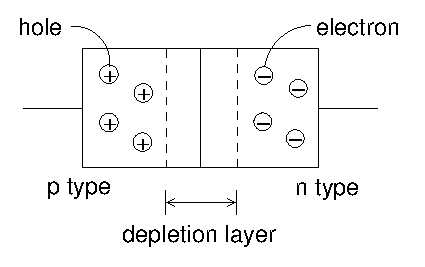
\includegraphics[clip,width=4cm]{1999phy4-7.eps}\\
図7
\end{center}
\begin{center}
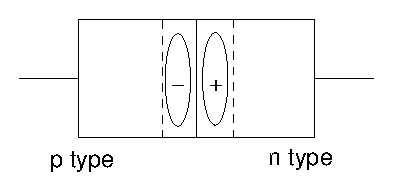
\includegraphics[clip,width=4cm]{1999phy4-8.eps}\\
図8
\end{center}
\end{minipage}

\SubSubAnswer
図9のような設定であるので\\
\begin{minipage}{.4\linewidth}
\[
\left\{
\begin{array}{l}
P_0 = \sigma T^4 \cdot 4 \pi R^2 \\
I_0 = \frac{P_0}{4 \pi L^2} = \sigma T^4 \cdot \frac{R^2}{L^2}
\end{array}
\right.
\]
に数値を代入して
\[
\left\{
\begin{array}{l}
P_0 = 4.0 \times 10^{26} \ \mathrm{[W]} \\
I_0 = 1.4 \times 10^3 \ \mathrm{[W/m^2]}
\end{array}
\right.
\]

\end{minipage}
\hspace{.1\linewidth}
\begin{minipage}{.4\linewidth}
\begin{center}
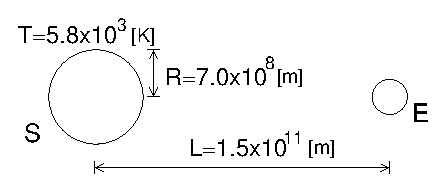
\includegraphics[clip,width=\linewidth]{1999phy4-9.eps}\\
図9
\end{center}
\end{minipage}

\SubSubAnswer
図10のように5つにブロック分けをすると
\begin{eqnarray*}
 (太陽電池の出力電流) 
 &=& \int \d{\nu}\ (光子数) \times (量子効率) \times (素電荷)\\
 &=& (面積) \times 10^8 \times \left( \sum _{ブロック} (単位面積の光子数) \times \times (量子効率) \right) \\
 &=& (0.05)^2 \times 10^8 \times 1.6\times10^{-19}\{(12 \times 10^{12}) \times  0.4 \\
 & & + (9 \times 10^{12}) \times 0.9 + (6 \times 10^{12}) \times 0.9 \\
 & & + (4 \times 10^{12}) \times 0.8 + (2 \times 10^{12}) \times 0.6 \} \\
 &=& 0.908 \approx 0.9 \Unit{[A]}
\end{eqnarray*}

\begin{center}
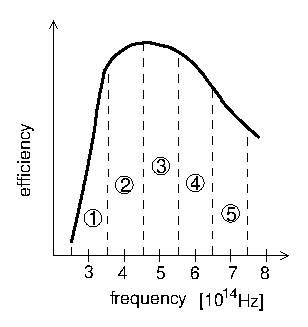
\includegraphics[clip]{1999phy4-10.eps} \\
図10
\end{center}

\SubSubAnswer
太陽光の一部が大気に吸収、反射されたため。
\end{subsubanswers}
\end{subanswers}
\end{answer}


\end{document}

